%%%%%%%%%%%%%%%%%%%%%%%%%%%%%%%%%%%%%%%%%%%%%%%%%%%%%%%%%%%%%%%%%%%%%%%%%%%
\chapter{Introduction}
%%%%%%%%%%%%%%%%%%%%%%%%%%%%%%%%%%%%%%%%%%%%%%%%%%%%%%%%%%%%%%%%%%%%%%%%%%%
The A* pathfinding algorithm is a best-first pathfinding algotithm for graphs commonly used 
for graph traversal applications such as artificial intelligence, video games, flight paths, and more.
However, while most games are written in an imperative and object-oriented language such as C\#, C++, and 
JavaScript, it is possible to write video games in a functional language using a reactive 
functional programming approach.\cite{Cheong2006} Likewise, the need for other correct critical software 
led organizations such as NASA to use Haskell\cite{HaskellSite}, a purely-functional programming language, to 
be used in systems where high-level assurance and provable programs are a must.\cite{NasaCopilot2020}

This paper assumes concrete differences between \emph{parallel} and \emph{concurrent} where the former 
is defined to be a hardware feature of having multiple processors or cores to compute a problem whereas the 
latter is defined to be a software-based approach to decrease the impact of computation bottlenecks by 
switching between different computations when a computation takes too long.\cite{SilberschatzGalvin2012} One of the major challenges 
of parallel programming is controlling the order of execution to prevent \emph{race conditions}, 
which can often lead to bugs and are hard to maintain. However, since pure functional languages, such as Haskell,
have no mutability and computations lead to the same result regardless of the order, they are a perfect candidate 
for writing parallel programs.\cite{Hammond2011}
This research aims to find a parallel implementation of the existing A* pathfinding algorithms using a 
purely-functional setting with attention to program performance. In turn, this helps in the advancement 
of different functional programming approaches for parallel graph computations which could eventually lead
to critical systems to use a more provable programming language.


% The Shortest Common Superstring (SCS) problem, known to be NP-Complete,
% seeks the shortest string that contains all strings from a given set.
% In this paper, we provide the summary of the problem and some of its characteristics.

% The SCS problem has been extensively studied for its
% applications in string compression and DNA sequence assembly \cite{Ma2009}.

% The superstring problem has applications to data storage,
%  specifically, data (string) compression \cite{Gallant1980}. 
% In many programming languages, a character string may be 
% represented by a pointer to that string. 
% The problem for the compiler is to arrange strings 
% so that they may be ``overlapped'' as much as possible.

% DNA sequence assembly is another  problem to which an SCS algorithm is known to apply.
% The $sequencing$ problem in molecular biology is to ``read'' a string of DNA,
% which can be viewed as a string over the alphabet \{A,C,G,T\}. Sequencing produces such a large number of fragments that
% almost all genome positions are covered by many fragments. This short fragments
% thus have large overlaps between other pieces. Hence, they can be given as an input to SCS algorithm.
% Figure \ref{fig:dna-overlap} shows an overlap graph consisting DNA reads (or fragments) as nodes. 



% \begin{figure*}
% \centering
% \fbox{
% \scalebox{0.65}{
% 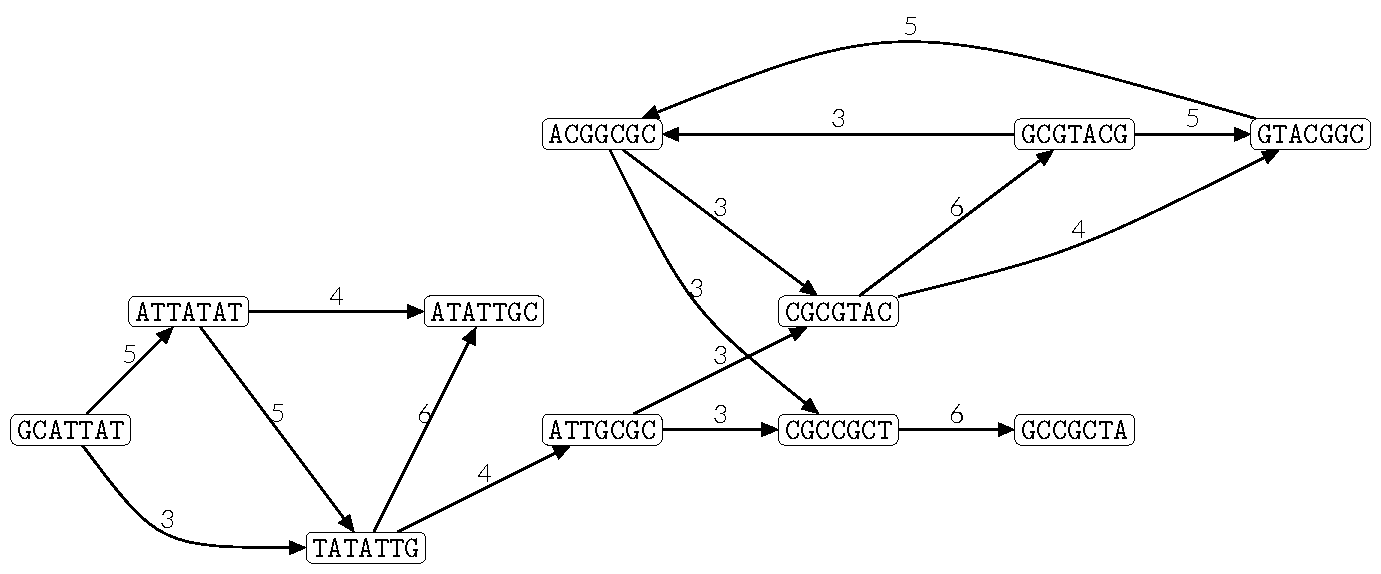
\includegraphics{fig-overlaps-dns-example}
% }}
% \caption{Sample overlap graph with each adjacent nodes 
% having at least $k = 3$ overlaps. The original string is \texttt{GCATTATATATTGCGCGTACGGCGCCGCTACA}.}
% \label{fig:dna-overlap}
% \end{figure*}	

% In \cite{Ma2009}'s paper, SCS was used to analyze DNA sequence assembly using
% a greedy algorithm. 

\section{Project Context}
The Therac-25 medical radiation machine caused at overdose accidents in which it harmed at least six patients using the machine.
One of the main causes of the problem was due to poor software engineering practices and that testing the software was
not enough.\cite{Therac1}
Most critical systems such as flight software, navigation, and military software is written in languages that may not guarantee 
correctness of programs such as C where adding $1$ to an \verb|int8| whose value is $65535$ may cause the program to show the 
incorrect sum of $-65536$. These kinds of problems often lead to software crashes and cause unexpected failures.
Also, the video game industry is dominated by imperative programming languages. However, due to the rise of 
languages such as TypeScript and PureScript, and frameworks such as ReactJS which favors a reactive functional programming approach,
it is not fanciful to say that games might start being written in the functional style as well. 

However, the functional style of programming has a different set of problems compared to its imperative counterpart such as 
obscurity for some programmers (though, this is subjective) and increased space complexity for the same algorithm. Multiple 
algorithms for the imperative approaches may not translate well and may even increase the time and space complexity for the functional 
approach due to its nature of copying the data structure instead of iterating over.


The advantages of functional programming lies with its \emph{referential transparency} which means that 
a function definition or a variable will never change its definition throughout the runtime of the program.\cite{Kesseler1996,Hammond2011}
Hence, mathematically proving functional programs might be easier and can be aided by proof assistants such as  
Coq or Agda.\cite{Breitner2018,SpectorZabusky2018,ElBakouny2017} Likewise, splitting functions into smaller functions and 
reasoning about those smaller components much like lemmas would mean that functions would be modular and composed of 
proven subfunctions.\cite{AbelBenkeBove2005,Hughes1989} Hence, functional programming languages are 
excellent candidates for parallel programming since the languages do not have mutable states and are therefore, instances of
shared variables are abstracted away from the programmer. Similarly, the order of execution of pure functions does not matter 
as the program will still yield the same results.\cite{Kesseler1996} 
A parallel and purely-functional approach to the A* algorithm would eventually lead to more applications such as
shortest distance in a map, flight paths, web server searching, and more to use a more provable and type-safe language which 
could lead to less system failures and high availability.

\section{Purpose and Description}

This research aims to utilize the existing parallel A* pathfinding algorithm
\cite{ZaghloulAlJami2017,WeinstockHolladay}
and find a way to develop a reasonably-efficient purely-functional 
implementation of the algorithm using parallel data structures such 
as STMs or MVars\cite{Marlow2013}.  

The A* Pathfinding algorithm is used heavily in video games, telephone traffic, 
and other graph traversal problems\cite{HartNilssonRaphael1968}. This research 
aims to aid in the development of video games and in developing safer critical systems 
with stricter error-checking and type safety.\cite{NasaCopilot2020} 

\section{Objectives}
The main objective of the research is to develop functional implementations of two different
parallel A* implementations. The research will be done using Haskell and Rust as a comparative metric for
imperative languages. Likewise, concrete comparisons between the number of cores and logical threads will be 
used to measure the most efficient runtime and space complexity of both algorithms.

The researchers aim to complete the following tasks:
\begin{itemize}
    \item Model multiple combinatorial problems such as the $n$-queens problem and Sudoku. These problems 
        may or may not have different problem sizes.
    \item A solver will be written both in Haskell, a laze purely-functional programming language, and Rust, 
        a relatively modern systems programming language that shares multiple features with Haskell.
    \item Two algorithms will be written in both languages and their performance will be recorded. The program
        Threadscope will be utilized for recording the performance of the Haskell solvers, such as thread and core 
        activities while the program is being run.
\end{itemize}

% The main objective of the research is to find an efficient parallel purely-functional implementation 
% of the A* pathfinding algorithm. The research will be done mostly in Haskell with some exceptions.
% Likewise, concrete comparisons between the number of cores and logical threads will be used to measure 
% the most efficient performance runtime and space complexity of the algorithm.

% The researchers aim to complete the following specific tasks:
% \begin{itemize}
%     \item Write a \emph{generator} that will generate an arbitrary-sized maze. The maze should be relatively 
%         hard to solve without the aid of computers in a short amount of time.\cite{Buck2015}
%     \item And a \emph{solver} program that will be written in Haskell, a lazy purely-functional programming language,
%         for translating the output of the generator to a graph.\cite{HaskellSite}
%     \item The solver program should have a web-based user interface where the researchers can view the maze and how 
%         the solver program was able to solve it correctly.
%     \item Performance of the solution shall be measured by using ThreadScope to monitor the thread and core activities 
%         while the program is being run.\cite{ThreadScope}
% \end{itemize}
% \vfill\eject
\section{Scope and Limitations}

The research will only cover Haskell, though it may generalize to other functional languages that support a parallel 
and concurrent approach. Translation to other functional programming languages is not a priority and thus, the use 
of abstract machines or lambda calculus notation will not be used. The researches deem that using a pure functional language 
such as Haskell will enable it to generalize well even on impure languages such as LISP.
Also, only problems where solutions exist will be tested on. 

The concrete implementation and analysis is planned to be tested only on four CPUs such as Intel Core i7-9750H and AMD Ryzen 5 3500x.
Other CPU architectures are not planned to be tested on.